
\chapter{Generating novel isoform models}\label{ap:gen-novl-iso}

In this appendix, we describe our approach for generating novel gene isoform models. We first select a set of seed reference isoforms and introduce modifications that are well known to occur via alternative isoform regulation \textit{in vivo}. These modifications include the use of alternative 5' start sites, alternative 3' end sites, alternative splice donors and acceptors, exon skipping, intron retention, and the introduction of new exons and introns. In addition, we also introduce a new modification, termed \textit{subset} isoform, that drops exons from the reference isoform from the 5' end (Fig. \ref{fig:app-a-1}). Introduction of these novel subset isoforms increases the number of multi-mapping reads, making the process of assigning these reads to the correct isoform more complex. 

\begin{figure}[H]
    \centering
    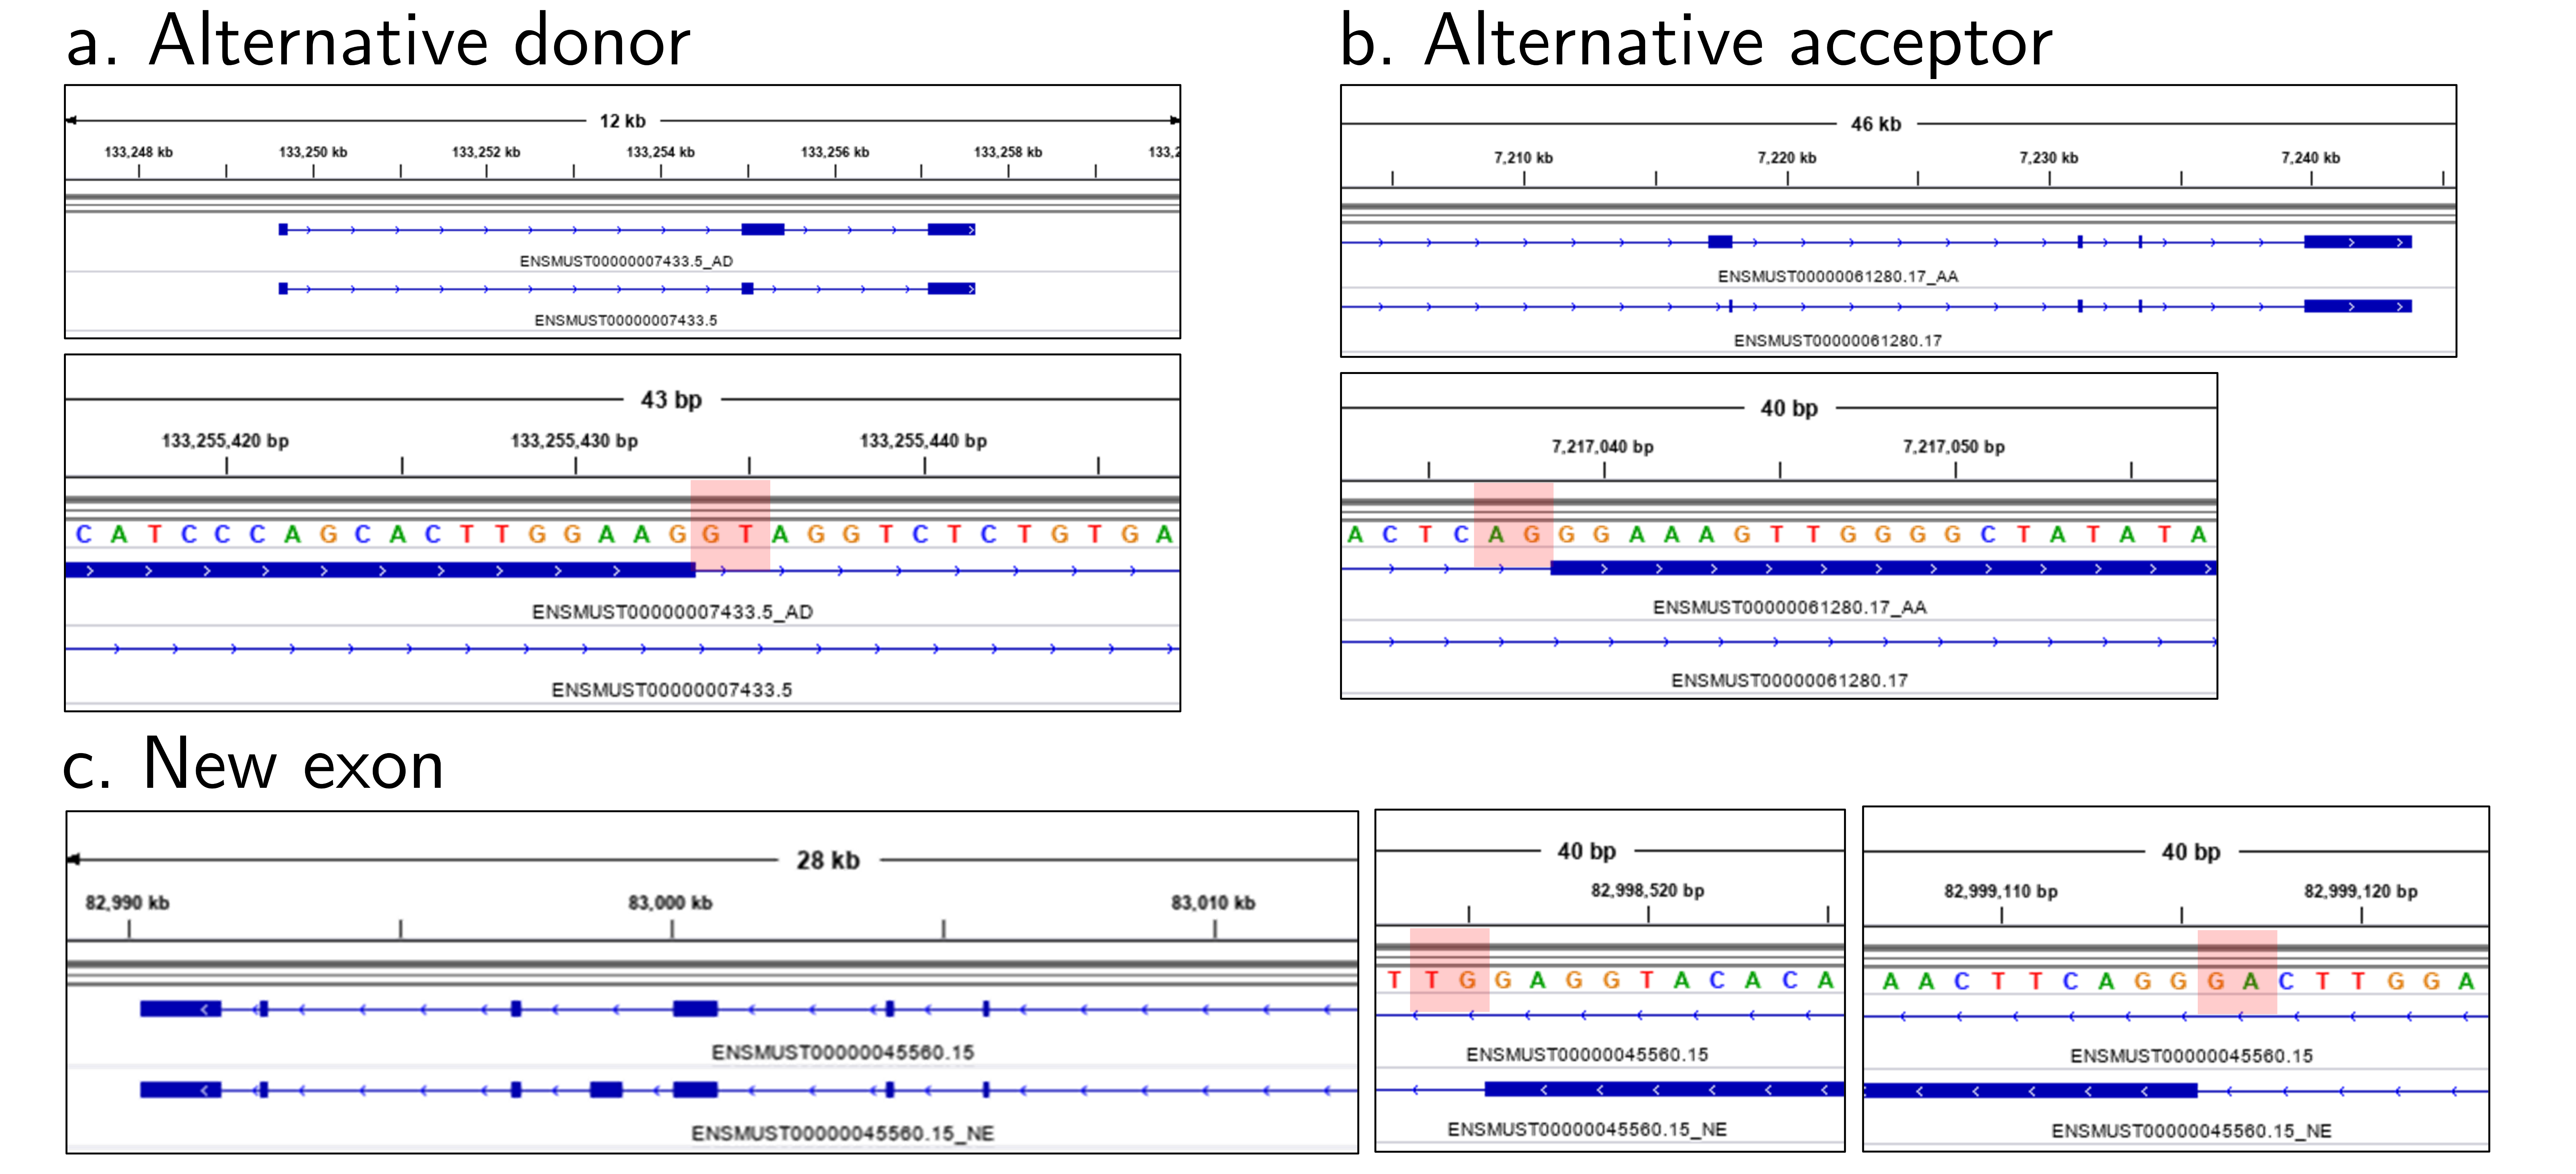
\includegraphics[width=\textwidth]{figures/app-a-1.png}
    \caption[Subset isoform modification]{Subset isoform modification. Exons from the 5' end of the reference isoform (blue) are removed to produce a truncated isoform comprising a subset of the exons of the original isoform.}
    \label{fig:app-a-1}
\end{figure}

Because the \texttt{minimap2} aligner uses splice site signals to map reads, we ensure that the generated novel isoform models conform to these splice site signals. We do so by performing splice site correction whenever necessary, i.e., for the alternative splice donor, alternative splice acceptor, new exon and new intron modifications (Fig. \ref{fig:app-a-2}). 

\begin{figure}[H]
    \centering
    \includegraphics[width=\textwidth]{figures/app-a-2.png}
    \caption[Splice site correction for novel isoform models]{Splice site correction for novel isoform models for the GT-AG motif. \textbf{a.} Alternative donor splice site. \textbf{b.} Alternative accept split site. \textbf{c.} New exon introduction.}
    \label{fig:app-a-2}
\end{figure}

\chapter{Simulating degraded reads}\label{ap:sim-deg-reads}

In this appendix, we describe our approach for simulating reads based on constant expected degradation. We select protein-coding isoforms and processed transcripts from GRCh38 annotation to simulate reads for. The distribution of counts follows a negative binomial distribution (parameterised here by the mean and rate), which is commonly used along with the Poisson distribution for modeling count data in RNA-seq. The negative binomial distribution has an added advantage of modeling overdispersion in the data, where the variance is greater than the mean. We note that the negative binomial distribution is equivalent to a mixture of Poisson distributions where the rate parameter is distributed according to a gamma distribution. 

To generate reads for a transcript of length $\mathrm{len}(j)$ given a degradation rate $d$, we first compute the maximum read length $\ell_\mathrm{max}=1/d$. The probability of generating a degraded read is $p_d=\min(\mathrm{len}(j)/\ell_\mathrm{max}, 1)$ and the probability of generating a full-length read is $1-p_d$. We now generate a read length with the following algorithm:
\begin{enumerate}
    \item Generate $U\sim Unif(0,1)$.
    \item If $U<p_d$, generate read length $\ell_i\sim Unif(0,\min(\mathrm{len}(j),\ell_\mathrm{max}))$.
    \item Otherwise, generate read length $\ell_i=\mathrm{len}(j)$
\end{enumerate}
For constant degradation, degraded reads follow a uniform distribution upper bounded by the length of the transcript isoform or the maximum read length, whichever is smaller. Once the read length $\ell_i$ is generated, we simply slice the transcript isoform sequence from the 3' end such that the resulting sequence is of length $\ell_i$. The reads simulated are thus perfect reads with 0\% error rate and no indels. 

\chapter{Proof of concavity of log-likelihood function}\label{sec:proof-log-lik}

Hello world.

\chapter{Derivations for variational distributions}\label{sec:variational-dist}

\begin{equation}
\begin{split}
    \log q(\bm{Z}) & = \mathbb{E}_{\bm\theta}\left[\log p(\bm{R},\bm{Z},\bm{\theta})\right] + \textrm{const.} \\
    & = \mathbb{E}_{\bm\theta}\left[\log p(\bm{R}\mid\bm{Z})\right] + \mathbb{E}_{\bm\theta}\left[\log p(\bm{Z}\mid\bm{\theta})\right] + \textrm{const.} \\
    & = \sum_i\sum_j z_{ij}\log\left[a_{ij}\cdot p(\ell_i\mid d_j,z_{ij}=1)\right] + \sum_i\sum_j z_{ij}\mathbb{E}_{\bm\theta}\left[\log\theta_j\right] + \textrm{const.}
\end{split}
\end{equation}

\chapter{Evaluation metrics}

\lipsum[32]

\chapter{Data and code availability}

We used long-read RNA-seq data from the SG-NEx project. Data is available at \url{https://github.com/GoekeLab/sg-nex-data}. 

Software for generating novel isoform models was written in \texttt{python} and is available at \url{https://github.com/jleechung/noviso}.

Software for simulating degraded reads was written in \texttt{python} and is available at \url{https://github.com/jleechung/shamread}. 

Software for our model for degradation-aware isoform quantification was written in \texttt{python} and is available at \url{https://github.com/jleechung/daiso}. 
